\subsection{Sampling design and estimands}
\label{sec:discovery-curves}
Large-budget \texttt{pass@k} evaluation can reveal differences hidden at smaller budgets \citep{yue2025rlvrlimit}. We evaluate sixteen problems from each of \texttt{Python}, \texttt{MathIR}, and \texttt{PantryPlan} at Levels~2 and~3.

Problems are selected independently of model outputs from the prompt-hint ablation population. Each has original and neutral wordings, with 64 responses per wording from each checkpoint or deployment. Eight-draw estimates use subsets of these same response pools. The initial Qwen2.5-0.5B-Instruct checkpoint has no training-seed replication. Dr.GRPO and Re:Dr use five matched seeds in \texttt{Python} and \texttt{MathIR} and two in \texttt{PantryPlan}. These checkpoints are trained at Level~2, so Level~3 measures transfer.

For a 64-draw pool, let $c$ be the number of correct outputs and $n_j$ the count of verified canonical key $j$. At $k\in\{1,2,4,8,16,32,64\}$, we average over all size-$k$ subsets without replacement:
\[
 P_k=1-\frac{\binom{64-c}{k}}{\binom{64}{k}},\qquad
 D_k=\sum_j\left[1-\frac{\binom{64-n_j}{k}}{\binom{64}{k}}\right],\qquad B_k=D_k-P_k.
\]
Here $P_k$ is the probability of at least one correct response, $D_k$ is the expected number of distinct verified modes, and $B_k$ is the expected number of modes beyond the first success. Infeasible numerator combinations are zero. Incorrect, empty, refused, and truncated responses remain in the pool; only verifier-accepted responses contribute keys. The curve points are correlated because they share a response pool and describe finite-sample discovery. The gains $G_P=P_{64}-P_8$, $G_D=D_{64}-D_8$, and $G_B=B_{64}-B_8$ distinguish improvements in first-success probability from the discovery of additional modes; they do not estimate complete unseen support.

We report strict-verifier results and a formatting-normalization sensitivity analysis that preserves every strict success and canonical key. Intervals use 20,000 whole-problem bootstrap replicates, paired across wordings and stratified by domain and level. Five-seed intervals also resample matched training seeds with shared problem indices; \texttt{PantryPlan} intervals condition on its two checkpoints. Each domain--level comparison contains sixteen problems, and intervals are unadjusted for multiple comparisons. Zero-width intervals indicate no observed resampled variation and do not establish equivalence.

For breadth at a fixed number of correct draws, we average over subsets of $m$ correct responses:
\[
 R_m=\sum_j\left[1-\frac{\binom{c-n_j}{m}}{\binom{c}{m}}\right].
\]
Paired comparisons require $c\ge m$ under both wordings. They therefore condition on observed success, without equating accuracy or estimating diversity for excluded problems.

Eligibility varies with $m$, method, and grading. Trained-checkpoint means weight seeds equally and are undefined if any seed lacks eligible prompts. Conditional intervals retain only bootstrap replicates in which the corresponding mean is defined.

The 64-draw summaries use two prompt weightings. Pooled collision $C$ divides the total number of equal-key correct pairs by the total number of correct pairs within each checkpoint or deployment; a prompt therefore receives weight proportional to $\binom{c}{2}$. Promptwise \pmd{} averages $1-\sum_j\binom{n_j}{2}/\binom{c}{2}$ equally over prompts with $c\ge2$. Each wording's absolute estimate uses its own eligible prompts, whereas the neutral-minus-original contrast $\Delta\pmd$ uses only jointly eligible prompts. Trained-checkpoint estimates then receive equal weight across seeds.

Support references use certified lower bounds $L\le M$: two valid modes in \texttt{Python}, five in \texttt{MathIR}, and the problem-specific certificate count in \texttt{PantryPlan}. Thus $1/L$ is an upper reference for collision under a uniform distribution over full support, and $L[1-(1-1/L)^m]$ is a lower reference for uniform expected breadth. These references describe uniform sampling; they do not bound model breadth, and observed distinct counts may exceed $L$.

In the tables, O/N denotes original/neutral wording, and $\Delta G_D$ is the neutral-minus-original discovery gain. $U$ denotes the uniform reference under the corresponding weighting. $E_O/E_N$ count separately eligible checkpoint--problem pairs with $c\ge2$; $Q_O/Q_N$ count correct response pairs. The counts sum across checkpoints, whereas the estimates weight checkpoints equally. Separate eligibility counts do not give the size of the jointly eligible population used for a contrast.


\begin{table}[!htbp]
\centering\scriptsize
\setlength{\tabcolsep}{3pt}
\caption{\textbf{Discovery gains from eight to 64 draws.} Strict verification; O/N denotes original/neutral wording. Each row reports sixteen problems for one deployment, domain, and level. Intervals resample paired problems, with no replication across model training seeds.}
\label{tab:discovery-gains-frontier-strict}
\resizebox{\linewidth}{!}{%
\begin{tabular}{llrrrr}
\toprule
Model & Domain/level & $G_P$: O/N & $G_D$: O/N & $G_B$: O/N & $\Delta G_D$ [95\%] \\
\midrule
GPT-5.4 & \texttt{Python} L2 & $0.014/0.000$ & $2.017/3.051$ & $2.003/3.051$ & $+1.033\;[-0.044,+2.371]$ \\
GPT-5.6 Sol & \texttt{Python} L2 & $0.000/0.405$ & $0.000/0.866$ & $0.000/0.462$ & $+0.866\;[+0.545,+1.231]$ \\
Grok 4.3 & \texttt{Python} L2 & $0.000/0.000$ & $0.667/1.013$ & $0.667/1.013$ & $+0.346\;[-0.583,+1.128]$ \\
GPT-5.4 & \texttt{Python} L3 & $0.025/0.000$ & $2.100/2.340$ & $2.076/2.340$ & $+0.240\;[-0.379,+0.930]$ \\
GPT-5.6 Sol & \texttt{Python} L3 & $0.000/0.586$ & $0.000/0.759$ & $0.000/0.174$ & $+0.759\;[+0.581,+0.952]$ \\
Grok 4.3 & \texttt{Python} L3 & $0.000/0.000$ & $0.424/1.576$ & $0.424/1.576$ & $+1.152\;[+0.640,+1.689]$ \\
GPT-5.4 & \texttt{MathIR} L2 & $0.043/0.042$ & $0.043/0.909$ & $0.000/0.868$ & $+0.867\;[+0.587,+1.111]$ \\
GPT-5.6 Sol & \texttt{MathIR} L2 & $0.027/0.004$ & $0.027/0.686$ & $0.000/0.682$ & $+0.659\;[+0.416,+0.888]$ \\
Grok 4.3 & \texttt{MathIR} L2 & $0.000/0.001$ & $0.223/0.322$ & $0.223/0.321$ & $+0.099\;[-0.226,+0.438]$ \\
GPT-5.4 & \texttt{MathIR} L3 & $0.000/0.000$ & $0.055/0.663$ & $0.055/0.663$ & $+0.609\;[+0.342,+0.888]$ \\
GPT-5.6 Sol & \texttt{MathIR} L3 & $0.000/0.000$ & $0.000/0.515$ & $0.000/0.515$ & $+0.515\;[+0.318,+0.714]$ \\
Grok 4.3 & \texttt{MathIR} L3 & $0.000/0.000$ & $0.167/0.805$ & $0.167/0.805$ & $+0.638\;[+0.348,+0.935]$ \\
GPT-5.4 & \texttt{PantryPlan} L2 & $0.001/0.015$ & $1.158/2.583$ & $1.156/2.568$ & $+1.426\;[+0.423,+2.641]$ \\
GPT-5.6 Sol & \texttt{PantryPlan} L2 & $0.086/0.101$ & $0.917/1.789$ & $0.831/1.688$ & $+0.872\;[+0.245,+1.575]$ \\
Grok 4.3 & \texttt{PantryPlan} L2 & $0.000/0.000$ & $1.022/3.377$ & $1.022/3.377$ & $+2.354\;[+1.592,+3.123]$ \\
GPT-5.4 & \texttt{PantryPlan} L3 & $0.000/0.002$ & $1.666/3.219$ & $1.666/3.218$ & $+1.553\;[+0.776,+2.367]$ \\
GPT-5.6 Sol & \texttt{PantryPlan} L3 & $0.032/0.129$ & $1.625/1.842$ & $1.592/1.713$ & $+0.217\;[-0.489,+0.921]$ \\
Grok 4.3 & \texttt{PantryPlan} L3 & $0.000/0.000$ & $1.810/4.466$ & $1.810/4.466$ & $+2.656\;[+1.698,+3.640]$ \\
\bottomrule
\end{tabular}}
\end{table}

\begin{table}[!htbp]
\centering\scriptsize
\setlength{\tabcolsep}{3pt}
\caption{\textbf{Discovery gains from eight to 64 draws.} Formatting normalization; O/N denotes original/neutral wording. Each row reports sixteen problems for one deployment, domain, and level. Intervals resample paired problems, with no replication across model training seeds.}
\label{tab:discovery-gains-frontier-normalized-secondary}
\resizebox{\linewidth}{!}{%
\begin{tabular}{llrrrr}
\toprule
Model & Domain/level & $G_P$: O/N & $G_D$: O/N & $G_B$: O/N & $\Delta G_D$ [95\%] \\
\midrule
GPT-5.4 & \texttt{Python} L2 & $0.000/0.000$ & $2.156/3.216$ & $2.156/3.216$ & $+1.060\;[-0.071,+2.386]$ \\
GPT-5.6 Sol & \texttt{Python} L2 & $0.008/0.010$ & $0.113/0.794$ & $0.105/0.784$ & $+0.681\;[+0.351,+1.066]$ \\
Grok 4.3 & \texttt{Python} L2 & $0.000/0.000$ & $0.667/1.013$ & $0.667/1.013$ & $+0.346\;[-0.583,+1.128]$ \\
GPT-5.4 & \texttt{Python} L3 & $0.000/0.000$ & $2.431/2.604$ & $2.431/2.604$ & $+0.173\;[-0.657,+1.075]$ \\
GPT-5.6 Sol & \texttt{Python} L3 & $0.011/0.007$ & $0.120/0.490$ & $0.109/0.483$ & $+0.370\;[+0.112,+0.674]$ \\
Grok 4.3 & \texttt{Python} L3 & $0.000/0.000$ & $0.424/1.576$ & $0.424/1.576$ & $+1.152\;[+0.640,+1.689]$ \\
GPT-5.4 & \texttt{MathIR} L2 & $0.043/0.042$ & $0.043/0.909$ & $0.000/0.868$ & $+0.867\;[+0.587,+1.111]$ \\
GPT-5.6 Sol & \texttt{MathIR} L2 & $0.027/0.004$ & $0.027/0.686$ & $0.000/0.682$ & $+0.659\;[+0.416,+0.888]$ \\
Grok 4.3 & \texttt{MathIR} L2 & $0.000/0.001$ & $0.223/0.322$ & $0.223/0.321$ & $+0.099\;[-0.226,+0.438]$ \\
GPT-5.4 & \texttt{MathIR} L3 & $0.000/0.000$ & $0.055/0.663$ & $0.055/0.663$ & $+0.609\;[+0.342,+0.888]$ \\
GPT-5.6 Sol & \texttt{MathIR} L3 & $0.000/0.000$ & $0.000/0.515$ & $0.000/0.515$ & $+0.515\;[+0.318,+0.714]$ \\
Grok 4.3 & \texttt{MathIR} L3 & $0.000/0.000$ & $0.167/0.805$ & $0.167/0.805$ & $+0.638\;[+0.348,+0.935]$ \\
GPT-5.4 & \texttt{PantryPlan} L2 & $0.001/0.015$ & $1.158/2.583$ & $1.156/2.568$ & $+1.426\;[+0.423,+2.641]$ \\
GPT-5.6 Sol & \texttt{PantryPlan} L2 & $0.004/0.004$ & $0.954/1.834$ & $0.950/1.830$ & $+0.880\;[+0.237,+1.547]$ \\
Grok 4.3 & \texttt{PantryPlan} L2 & $0.000/0.000$ & $1.022/3.377$ & $1.022/3.377$ & $+2.354\;[+1.592,+3.123]$ \\
GPT-5.4 & \texttt{PantryPlan} L3 & $0.000/0.002$ & $1.666/3.219$ & $1.666/3.218$ & $+1.553\;[+0.776,+2.367]$ \\
GPT-5.6 Sol & \texttt{PantryPlan} L3 & $0.001/0.020$ & $1.586/2.462$ & $1.585/2.443$ & $+0.877\;[+0.272,+1.436]$ \\
Grok 4.3 & \texttt{PantryPlan} L3 & $0.000/0.000$ & $1.810/4.466$ & $1.810/4.466$ & $+2.656\;[+1.698,+3.640]$ \\
\bottomrule
\end{tabular}}
\end{table}

\begin{figure}[!htbp]

\centering

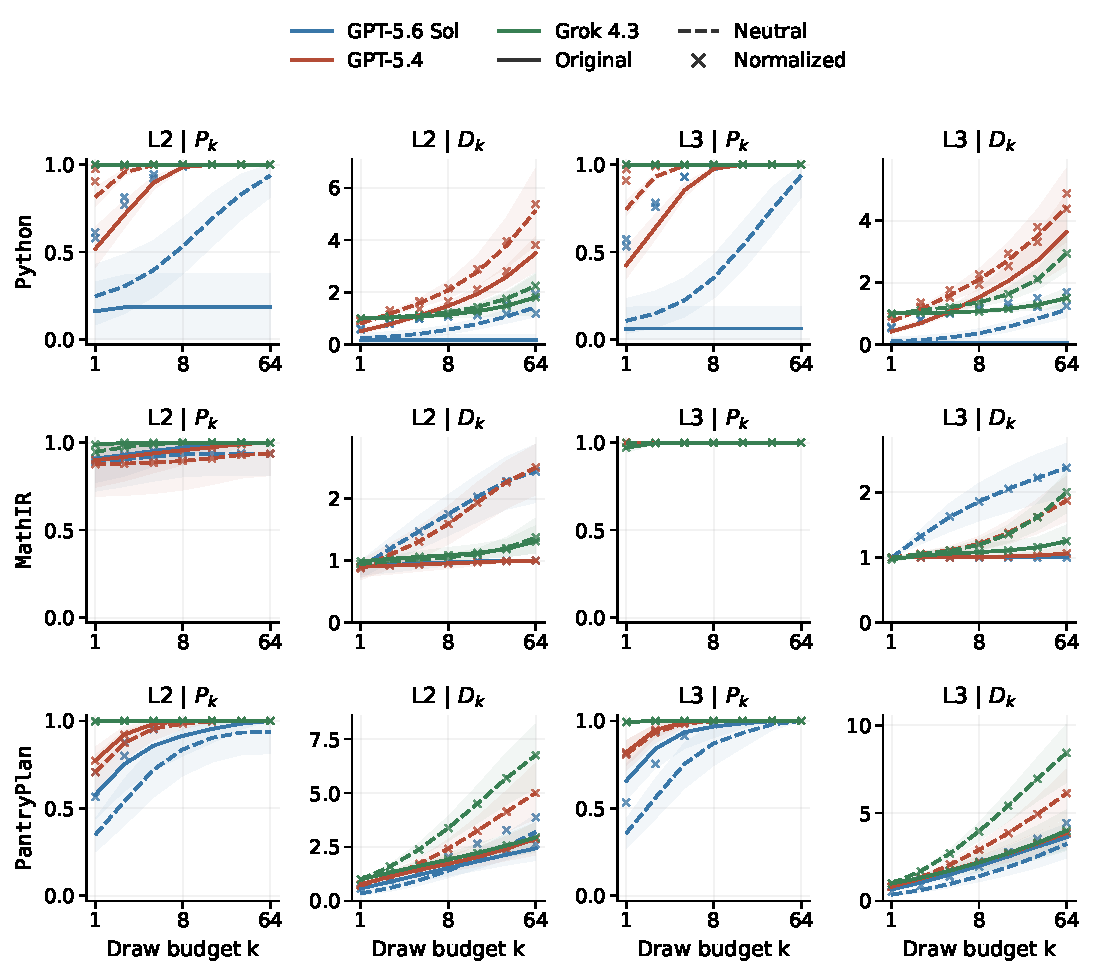
\includegraphics[width=\linewidth,height=0.72\textheight,keepaspectratio]{figures/modebench_discovery_curves_frontier.pdf}

\caption{\textbf{Additional draws reveal solution modes beyond early success.} Hosted deployments; rows show \texttt{Python}, \texttt{MathIR}, and \texttt{PantryPlan}, with paired $P_k$ and $D_k$ columns for Levels~2 and~3. Curves show pass probability $P_k$ and distinct verified modes $D_k$ against draw budget $k$, obtained by averaging over size-$k$ subsets within sixteen 64-draw problem pools per domain and level. Colours identify deployments; solid/dashed lines denote original/neutral wording. Lines use strict verification, crosses formatting normalization, and shading pointwise 95\% bootstrap intervals. Intervals resample paired problems within each domain and level and condition on the deployment.}

\label{fig:discovery-curves-frontier}

\end{figure}

\begin{table}[!htbp]
\centering\scriptsize
\setlength{\tabcolsep}{3pt}
\caption{\textbf{Pair weighting changes the summary of correct-solution diversity.} Strict 64-draw estimates for hosted deployments. Collision $C$ weights prompts by their number of correct pairs; \pmd{} weights eligible prompts equally. Absolute estimates for each wording use their own eligible prompts, whereas $\Delta\pmd$ uses only jointly eligible prompts. Thus $\Delta\pmd$ need not equal the difference between the displayed absolute estimates, and $E_O/E_N$ are separate eligibility counts. Each deployment is fixed; intervals resample paired problems.}
\label{tab:discovery-breadth-frontier}
\resizebox{\linewidth}{!}{%
\begin{tabular}{llrrrrrrrrr}
\toprule
Model & Domain/level & $C_O$ & $C_N$ & $\pmd_O$ & $\pmd_N$ & $U^{C}_O$ & $U^{\pmd}_O$ & $E_O/E_N$ & $Q_O/Q_N$ & $\Delta\pmd$ [95\%] \\
\midrule
GPT-5.4 & \texttt{Python} L2 & $0.790$ & $0.665$ & $0.257$ & $0.341$ & $0.500$ & $0.500$ & 16/16 & 10374/21720 & $+0.084\;[-0.006,+0.186]$ \\
GPT-5.6 Sol & \texttt{Python} L2 & $1.000$ & $0.974$ & $0.000$ & $0.184$ & $0.500$ & $0.500$ & 3/13 & 4467/6074 & $+0.021\;[+0.000,+0.032]$ \\
Grok 4.3 & \texttt{Python} L2 & $0.963$ & $0.938$ & $0.037$ & $0.062$ & $0.500$ & $0.500$ & 16/16 & 32256/32256 & $+0.025\;[+0.002,+0.048]$ \\
GPT-5.4 & \texttt{Python} L3 & $0.732$ & $0.620$ & $0.334$ & $0.384$ & $0.500$ & $0.500$ & 16/16 & 6747/18043 & $+0.050\;[-0.026,+0.128]$ \\
GPT-5.6 Sol & \texttt{Python} L3 & $1.000$ & $0.966$ & $0.000$ & $0.130$ & $0.500$ & $0.500$ & 1/10 & 1953/2097 & $+0.031\;[+0.031,+0.031]$ \\
Grok 4.3 & \texttt{Python} L3 & $0.981$ & $0.893$ & $0.019$ & $0.107$ & $0.500$ & $0.500$ & 16/16 & 32193/32256 & $+0.087\;[+0.041,+0.154]$ \\
GPT-5.4 & \texttt{MathIR} L2 & $1.000$ & $0.756$ & $0.000$ & $0.228$ & $0.200$ & $0.800$ & 16/15 & 28440/28227 & $+0.228\;[+0.161,+0.302]$ \\
GPT-5.6 Sol & \texttt{MathIR} L2 & $1.000$ & $0.678$ & $0.000$ & $0.302$ & $0.200$ & $0.800$ & 16/15 & 28645/28377 & $+0.302\;[+0.200,+0.402]$ \\
Grok 4.3 & \texttt{MathIR} L2 & $0.968$ & $0.985$ & $0.033$ & $0.014$ & $0.200$ & $0.800$ & 16/16 & 31600/29677 & $-0.020\;[-0.076,+0.017]$ \\
GPT-5.4 & \texttt{MathIR} L3 & $0.998$ & $0.944$ & $0.002$ & $0.056$ & $0.200$ & $0.800$ & 16/16 & 32256/32256 & $+0.054\;[+0.027,+0.087]$ \\
GPT-5.6 Sol & \texttt{MathIR} L3 & $1.000$ & $0.676$ & $0.000$ & $0.324$ & $0.200$ & $0.800$ & 16/16 & 32256/32256 & $+0.324\;[+0.208,+0.432]$ \\
Grok 4.3 & \texttt{MathIR} L3 & $0.966$ & $0.949$ & $0.033$ & $0.051$ & $0.200$ & $0.800$ & 16/16 & 30520/32193 & $+0.019\;[-0.046,+0.064]$ \\
GPT-5.4 & \texttt{PantryPlan} L2 & $0.680$ & $0.499$ & $0.252$ & $0.483$ & $0.069$ & $0.934$ & 16/16 & 20097/17436 & $+0.231\;[+0.069,+0.395]$ \\
GPT-5.6 Sol & \texttt{PantryPlan} L2 & $0.674$ & $0.624$ & $0.275$ & $0.474$ & $0.076$ & $0.934$ & 16/15 & 12941/5001 & $+0.180\;[+0.058,+0.327]$ \\
Grok 4.3 & \texttt{PantryPlan} L2 & $0.684$ & $0.412$ & $0.315$ & $0.589$ & $0.066$ & $0.934$ & 16/16 & 32005/32193 & $+0.274\;[+0.143,+0.411]$ \\
GPT-5.4 & \texttt{PantryPlan} L3 & $0.546$ & $0.392$ & $0.431$ & $0.610$ & $0.065$ & $0.937$ & 16/16 & 22332/21975 & $+0.179\;[+0.103,+0.257]$ \\
GPT-5.6 Sol & \texttt{PantryPlan} L3 & $0.566$ & $0.652$ & $0.422$ & $0.441$ & $0.061$ & $0.937$ & 16/16 & 15229/4946 & $+0.019\;[-0.136,+0.172]$ \\
Grok 4.3 & \texttt{PantryPlan} L3 & $0.673$ & $0.294$ & $0.330$ & $0.703$ & $0.063$ & $0.937$ & 16/16 & 31830/31881 & $+0.373\;[+0.224,+0.523]$ \\
\bottomrule
\end{tabular}}
\end{table}

\begin{figure}[!htbp]

\centering

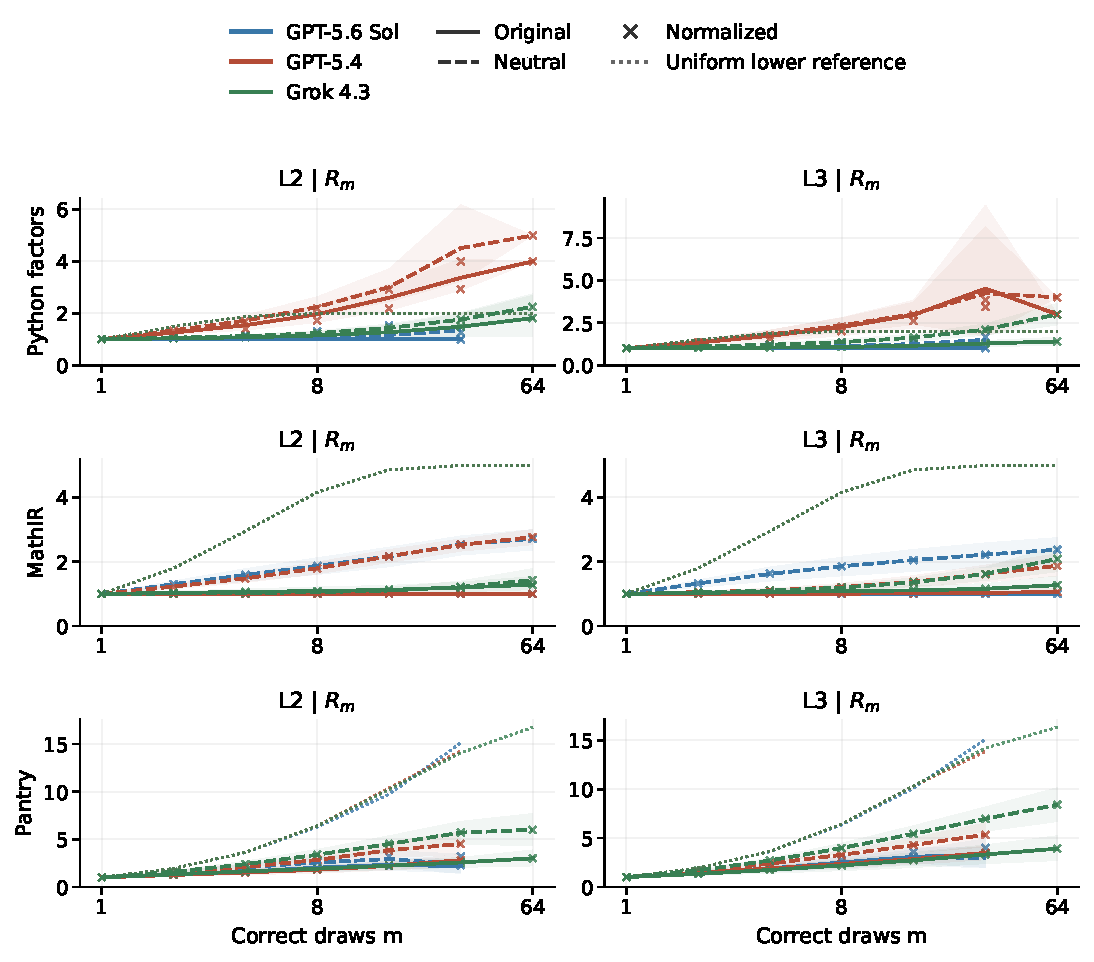
\includegraphics[width=\linewidth,height=0.66\textheight,keepaspectratio]{figures/modebench_discovery_correct_budget_frontier.pdf}

\caption{\textbf{Neutral wording broadens GPT solutions in \texttt{MathIR} at fixed correct-draw budgets.} Hosted deployments; rows show \texttt{Python}, \texttt{MathIR}, and \texttt{PantryPlan}, and columns Levels~2 and~3. Curves show $R_m$, the expected number of distinct verified modes in $m$ correct draws, on prompts with at least $m$ correct outputs under both wordings. Eligibility varies with $m$, method, and grading; gaps mark undefined means. Dotted lines give uniform lower references on prompts eligible under strict grading in both wordings, with the same prompt and checkpoint weighting as the strict curves. Colours identify deployments; solid/dashed lines denote original/neutral wording. Lines use strict verification, crosses formatting normalization, and shading pointwise 95\% bootstrap intervals. Intervals resample paired problems within each domain and level and condition on the deployment.}

\label{fig:discovery-correct-budget-frontier}

\end{figure}

\begin{table}[!htbp]
\centering\scriptsize
\setlength{\tabcolsep}{3pt}
\caption{\textbf{Discovery gains from eight to 64 draws.} Strict verification; O/N denotes original/neutral wording. Qwen2.5-0.5B-Instruct checkpoint means use five training seeds in \texttt{Python} and \texttt{MathIR} and two in \texttt{PantryPlan}; $s=1$ denotes the single initial checkpoint. Five-seed intervals resample seeds and paired prompts; \texttt{PantryPlan} intervals condition on its two checkpoints. Formatting normalization leaves every Qwen estimate unchanged.}
\label{tab:discovery-gains-local-strict}
\resizebox{\linewidth}{!}{%
\begin{tabular}{llrrrr}
\toprule
Model & Domain/level & $G_P$: O/N & $G_D$: O/N & $G_B$: O/N & $\Delta G_D$ [95\%] \\
\midrule
Dr.GRPO ($s=5$) & \texttt{Python} L2 & $0.000/0.000$ & $0.000/0.000$ & $0.000/0.000$ & $+0.000\;[+0.000,+0.000]$ \\
Initial ($s=1$) & \texttt{Python} L2 & $0.147/0.105$ & $0.303/0.165$ & $0.156/0.060$ & $-0.138\;[-0.217,-0.061]$ \\
Re:Dr ($s=5$) & \texttt{Python} L2 & $0.000/0.231$ & $0.058/0.463$ & $0.058/0.232$ & $+0.405\;[+0.185,+0.620]$ \\
Dr.GRPO ($s=5$) & \texttt{Python} L3 & $0.000/0.033$ & $0.000/0.033$ & $0.000/0.000$ & $+0.033\;[+0.000,+0.120]$ \\
Initial ($s=1$) & \texttt{Python} L3 & $0.218/0.096$ & $0.593/0.096$ & $0.376/0.000$ & $-0.497\;[-0.766,-0.270]$ \\
Re:Dr ($s=5$) & \texttt{Python} L3 & $0.000/0.239$ & $0.153/0.531$ & $0.153/0.292$ & $+0.379\;[+0.111,+0.678]$ \\
Dr.GRPO ($s=5$) & \texttt{MathIR} L2 & $0.021/0.017$ & $0.021/0.017$ & $0.000/0.000$ & $-0.004\;[-0.068,+0.045]$ \\
Initial ($s=1$) & \texttt{MathIR} L2 & $0.344/0.235$ & $0.344/0.235$ & $0.000/0.000$ & $-0.109\;[-0.383,+0.164]$ \\
Re:Dr ($s=5$) & \texttt{MathIR} L2 & $0.010/0.011$ & $0.010/0.011$ & $0.000/0.000$ & $+0.001\;[-0.036,+0.050]$ \\
Dr.GRPO ($s=5$) & \texttt{MathIR} L3 & $0.023/0.018$ & $0.026/0.018$ & $0.004/0.000$ & $-0.008\;[-0.065,+0.038]$ \\
Initial ($s=1$) & \texttt{MathIR} L3 & $0.254/0.246$ & $0.359/0.360$ & $0.105/0.114$ & $+0.001\;[-0.123,+0.095]$ \\
Re:Dr ($s=5$) & \texttt{MathIR} L3 & $0.064/0.056$ & $0.064/0.056$ & $0.000/0.000$ & $-0.008\;[-0.099,+0.059]$ \\
Dr.GRPO ($s=2$) & \texttt{PantryPlan} L2 & $0.332/0.323$ & $0.718/0.736$ & $0.386/0.414$ & $+0.018\;[-0.422,+0.433]$ \\
Initial ($s=1$) & \texttt{PantryPlan} L2 & $0.440/0.419$ & $0.857/0.955$ & $0.416/0.537$ & $+0.099\;[-0.201,+0.392]$ \\
Re:Dr ($s=2$) & \texttt{PantryPlan} L2 & $0.141/0.147$ & $0.415/0.429$ & $0.274/0.282$ & $+0.014\;[-0.123,+0.152]$ \\
Dr.GRPO ($s=2$) & \texttt{PantryPlan} L3 & $0.268/0.258$ & $0.949/1.025$ & $0.681/0.766$ & $+0.076\;[-0.237,+0.465]$ \\
Initial ($s=1$) & \texttt{PantryPlan} L3 & $0.259/0.384$ & $0.927/1.078$ & $0.668/0.694$ & $+0.151\;[-0.109,+0.399]$ \\
Re:Dr ($s=2$) & \texttt{PantryPlan} L3 & $0.204/0.149$ & $0.568/0.461$ & $0.364/0.312$ & $-0.107\;[-0.321,+0.098]$ \\
\bottomrule
\end{tabular}}
\end{table}

\begin{figure}[!htbp]

\centering

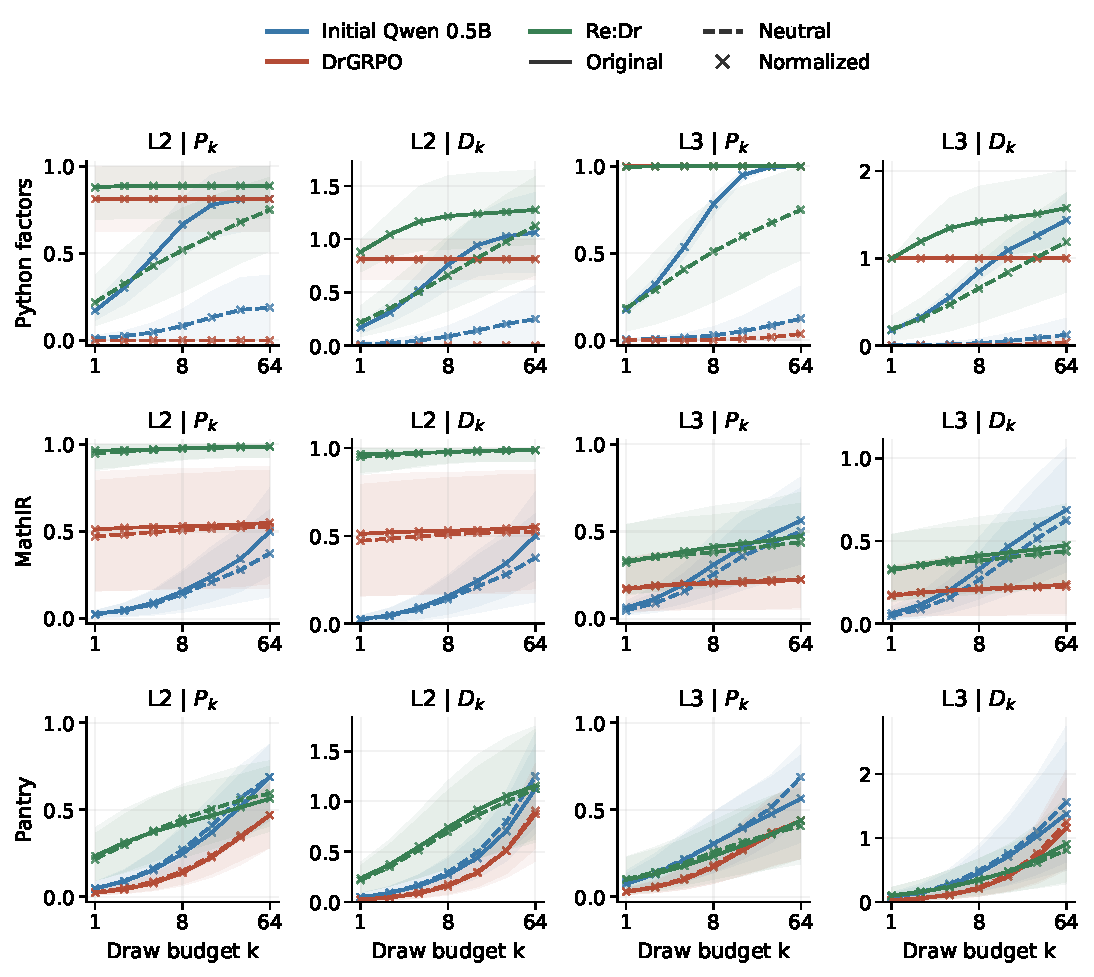
\includegraphics[width=\linewidth,height=0.72\textheight,keepaspectratio]{figures/modebench_discovery_curves_local.pdf}

\caption{\textbf{Additional draws reveal few new \texttt{MathIR} modes after training.} Qwen2.5-0.5B-Instruct checkpoints; rows show \texttt{Python}, \texttt{MathIR}, and \texttt{PantryPlan}, with paired $P_k$ and $D_k$ columns for Levels~2 and~3. Curves show pass probability $P_k$ and distinct verified modes $D_k$ against draw budget $k$, obtained by averaging over size-$k$ subsets within sixteen 64-draw problem pools per domain and level. Colours identify methods; solid/dashed lines denote original/neutral wording. Lines use strict verification, crosses formatting normalization, and shading pointwise 95\% bootstrap intervals. Means weight checkpoints equally: five training seeds in \texttt{Python} and \texttt{MathIR}, two in \texttt{PantryPlan}, and one initial checkpoint. Five-seed intervals resample seeds and paired problems; \texttt{PantryPlan} and initial intervals condition on the observed checkpoints for each method.}

\label{fig:discovery-curves-local}

\end{figure}

\begin{table}[!htbp]
\centering\scriptsize
\setlength{\tabcolsep}{3pt}
\caption{\textbf{Pair weighting changes the summary of correct-solution diversity.} Strict 64-draw estimates for Qwen2.5-0.5B-Instruct checkpoints. Collision $C$ weights prompts by their number of correct pairs; \pmd{} weights eligible prompts equally. Absolute estimates for each wording use their own eligible prompts, whereas $\Delta\pmd$ uses only jointly eligible prompts. Thus $\Delta\pmd$ need not equal the difference between the displayed absolute estimates, and $E_O/E_N$ are separate eligibility counts. Means weight checkpoints equally and are undefined if any seed lacks eligible prompts.}
\label{tab:discovery-breadth-local}
\resizebox{\linewidth}{!}{%
\begin{tabular}{llrrrrrrrrr}
\toprule
Model & Domain/level & $C_O$ & $C_N$ & $\pmd_O$ & $\pmd_N$ & $U^{C}_O$ & $U^{\pmd}_O$ & $E_O/E_N$ & $Q_O/Q_N$ & $\Delta\pmd$ [95\%] \\
\midrule
Dr.GRPO & \texttt{Python} L2 & $1.000$ & $--$ & $0.000$ & $--$ & $0.500$ & $0.500$ & 65/0 & 130977/0 & $--$ \\
Initial & \texttt{Python} L2 & $0.791$ & $0.875$ & $0.097$ & $0.167$ & $0.500$ & $0.500$ & 13/3 & 1270/24 & $-0.252\;[-0.395,+0.019]$ \\
Re:Dr & \texttt{Python} L2 & $0.809$ & $0.800$ & $0.191$ & $0.156$ & $0.500$ & $0.500$ & 71/53 & 140722/18289 & $-0.037\;[-0.139,+0.037]$ \\
Dr.GRPO & \texttt{Python} L3 & $1.000$ & $--$ & $0.000$ & $--$ & $0.500$ & $0.500$ & 80/0 & 161280/0 & $--$ \\
Initial & \texttt{Python} L3 & $0.875$ & $1.000$ & $0.101$ & $0.000$ & $0.500$ & $0.500$ & 16/1 & 1010/3 & $-0.513\;[-0.513,-0.513]$ \\
Re:Dr & \texttt{Python} L3 & $0.805$ & $0.797$ & $0.195$ & $0.227$ & $0.500$ & $0.500$ & 80/52 & 160275/12893 & $+0.030\;[-0.023,+0.117]$ \\
Dr.GRPO & \texttt{MathIR} L2 & $1.000$ & $1.000$ & $0.000$ & $0.000$ & $0.200$ & $0.800$ & 43/42 & 80766/74119 & $+0.000\;[+0.000,+0.000]$ \\
Initial & \texttt{MathIR} L2 & $1.000$ & $1.000$ & $0.000$ & $0.000$ & $0.200$ & $0.800$ & 3/3 & 64/64 & $+0.000\;[+0.000,+0.000]$ \\
Re:Dr & \texttt{MathIR} L2 & $1.000$ & $1.000$ & $0.000$ & $0.000$ & $0.200$ & $0.800$ & 79/79 & 155016/151485 & $+0.000\;[+0.000,+0.000]$ \\
Dr.GRPO & \texttt{MathIR} L3 & $0.980$ & $1.000$ & $0.038$ & $0.000$ & $0.200$ & $0.800$ & 16/18 & 24457/25393 & $-0.038\;[-0.202,+0.000]$ \\
Initial & \texttt{MathIR} L3 & $0.883$ & $0.912$ & $0.128$ & $0.162$ & $0.200$ & $0.800$ & 7/6 & 282/181 & $+0.013\;[-0.014,+0.052]$ \\
Re:Dr & \texttt{MathIR} L3 & $1.000$ & $1.000$ & $0.000$ & $0.000$ & $0.200$ & $0.800$ & 34/34 & 46891/50301 & $+0.000\;[+0.000,+0.000]$ \\
Dr.GRPO & \texttt{PantryPlan} L2 & $0.374$ & $0.276$ & $0.733$ & $0.780$ & $0.047$ & $0.953$ & 9/10 & 101/193 & $+0.220\;[-0.030,+0.470]$ \\
Initial & \texttt{PantryPlan} L2 & $0.849$ & $0.787$ & $0.587$ & $0.623$ & $0.052$ & $0.945$ & 7/10 & 212/178 & $-0.078\;[-0.300,+0.064]$ \\
Re:Dr & \texttt{PantryPlan} L2 & $0.600$ & $0.613$ & $0.343$ & $0.218$ & $0.051$ & $0.942$ & 16/18 & 10144/8510 & $-0.093\;[-0.220,+0.007]$ \\
Dr.GRPO & \texttt{PantryPlan} L3 & $0.203$ & $0.228$ & $0.808$ & $0.680$ & $0.047$ & $0.950$ & 10/12 & 134/165 & $-0.156\;[-0.359,+0.081]$ \\
Initial & \texttt{PantryPlan} L3 & $0.375$ & $0.313$ & $0.307$ & $0.341$ & $0.049$ & $0.945$ & 7/6 & 531/705 & $-0.017\;[-0.109,+0.091]$ \\
Re:Dr & \texttt{PantryPlan} L3 & $0.636$ & $0.666$ & $0.337$ & $0.198$ & $0.051$ & $0.941$ & 10/11 & 4006/3946 & $-0.112\;[-0.319,+0.008]$ \\
\bottomrule
\end{tabular}}
\end{table}

\begin{figure}[!htbp]

\centering

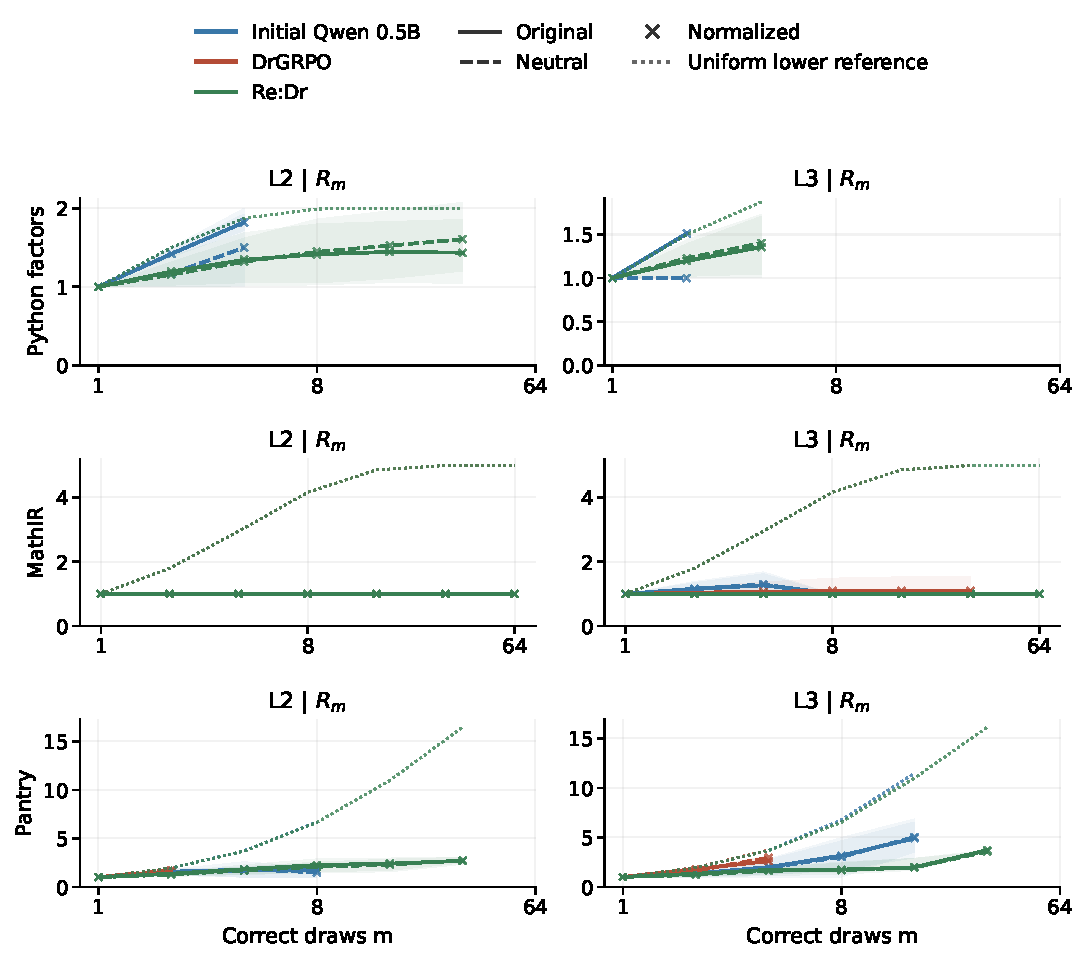
\includegraphics[width=\linewidth,height=0.66\textheight,keepaspectratio]{figures/modebench_discovery_correct_budget_local.pdf}

\caption{\textbf{\texttt{MathIR} correct solutions remain concentrated after training.} Qwen2.5-0.5B-Instruct checkpoints; rows show \texttt{Python}, \texttt{MathIR}, and \texttt{PantryPlan}, and columns Levels~2 and~3. Curves show $R_m$, the expected number of distinct verified modes in $m$ correct draws, on prompts with at least $m$ correct outputs under both wordings. Eligibility varies with $m$, method, and grading; gaps mark undefined means. Dotted lines give uniform lower references on prompts eligible under strict grading in both wordings, with the same prompt and checkpoint weighting as the strict curves. Colours identify methods; solid/dashed lines denote original/neutral wording. Lines use strict verification, crosses formatting normalization, and shading pointwise 95\% bootstrap intervals. Means weight checkpoints equally: five training seeds in \texttt{Python} and \texttt{MathIR}, two in \texttt{PantryPlan}, and one initial checkpoint. Five-seed intervals resample seeds and paired problems; \texttt{PantryPlan} and initial intervals condition on the observed checkpoints for each method.}

\label{fig:discovery-correct-budget-local}

\end{figure}
